
\let\negmedspace\undefined
\let\negthickspace\undefined
\documentclass[journal]{IEEEtran}
\usepackage[a5paper, margin=10mm, onecolumn]{geometry}
%\usepackage{lmodern} % Ensure lmodern is loaded for pdflatex
\usepackage{tfrupee} % Include tfrupee package
\setlength{\headheight}{1cm} % Set the height of the header box
\setlength{\headsep}{0mm}     % Set the distance between the header box and the top of the text
\usepackage{gvv-book}
\usepackage{gvv}
\usepackage{cite}
\usepackage{amsmath,amssymb,amsfonts,amsthm}
\usepackage{algorithmic}
\usepackage{graphicx}
\usepackage{textcomp}
\usepackage{xcolor}
\usepackage{txfonts}
\usepackage{listings}
\usepackage{enumitem}
\usepackage{mathtools}
\usepackage{gensymb}
\usepackage{comment}
\usepackage[breaklinks=true]{hyperref}
\usepackage{tkz-euclide} 
\usepackage{listings}
% \usepackage{gvv}                                        
\def\inputGnumericTable{}                                 
\usepackage[latin1]{inputenc}                                
\usepackage{color}                                            
\usepackage{array}                                            
\usepackage{longtable}                                       
\usepackage{calc}                                             
\usepackage{multirow}                                         
\usepackage{hhline}                                           
\usepackage{ifthen}                                           
\usepackage{lscape}
\renewcommand{\thefigure}{\theenumi}
\renewcommand{\thetable}{\theenumi}
\setlength{\intextsep}{10pt} % Space between text and floats
\numberwithin{equation}{enumi}
\numberwithin{figure}{enumi}
\renewcommand{\thetable}{\theenumi}
\begin{document}
\bibliographystyle{IEEEtran}
\title{Question 1-1.4-9p}
\author{EE24BTECH11041 - Mohit}
% \maketitle
% \newpage
% \bigskip
{\let\newpage\relax\maketitle}
\begin{enumerate}
	\item Let $\vec{A}\brak{4,2}$,$\vec{B}\brak{6,5}$ and $\vec{C}\brak{1,4}$ be the vertices of $\Delta$ $ABC$.Find the coordinates of points $\vec{Q}$ and $\vec{R}$ on medians $BE$ and $CF$ respectively such that $BQ:QE=2:1$ and $CR:RF=2:1$.
\end{enumerate}
\begin{table}[h!]    
  \centering
  \begin{tabular}[12pt]{ |c| c|}
    \hline
    \textbf{Variable} & \textbf{Description} \\ 
    \hline
    $\vec{x_1}$ & Point on circle \\
    \hline
    $\vec{x_2}$ & Point on circle \\
    \hline 
    $\vec{n}$ &  Equation of line on centre of circle lies \\
    \hline   
    \end{tabular}

  \caption{Variables Used}
  \label{tab10.5.3.9.1}
\end{table}
Solution:-\\
$\vec{F}$ is the mid point of $AB$\\
\begin{align}
	\vec{F}=\frac{A+B}{2}=\frac{\myvec{4\\2} + \myvec{6\\5}}{2}
=\myvec{5\\ \frac{7}{2}}
\end{align}
$\vec{E}$ is the mid point of $AC$\\
\begin{align}
	\vec{E}=\frac{A+C}{2}==\frac{\myvec{4\\2} + \myvec{1\\4}}{2}
=\myvec{\frac{5}{2}\\3}
\end{align}
By section formula,
\begin{align}
	\vec{R}=\frac{B+KA}{1+K}
\end{align}
It is given that $\frac{BQ}{QE}=\frac{2}{1}$\\
So,\\
\begin{align}
	\vec{Q}=\frac{B+2E}{1+2}=\frac{\myvec{6\\5} + 2\myvec{\frac{5}{2}\\3}}{3}=\myvec{\frac{11}{3}\\ \frac{11}{3}}
\end{align}
It is given that $\frac{CR}{RF}=\frac{2}{1}$\\
So,\\
\begin{align}
	\vec{R}=\frac{C+2F}{1+2}=\frac{\myvec{1\\4} + 2\myvec{5\\\frac{7}{2}}}{3}=\myvec{\frac{11}{3}\\ \frac{11}{3}}
\end{align}
Hence, Co-ordinates of $\vec{Q}$ and $\vec{R}$ are\\
\begin{align}
    \vec{Q}\brak{\frac{11}{3},\frac{11}{3}} \text{and}\ \vec{R}\brak{\frac{11}{3},\frac{11}{3}}
\end{align}
\begin{figure}[h!]
   \centering
   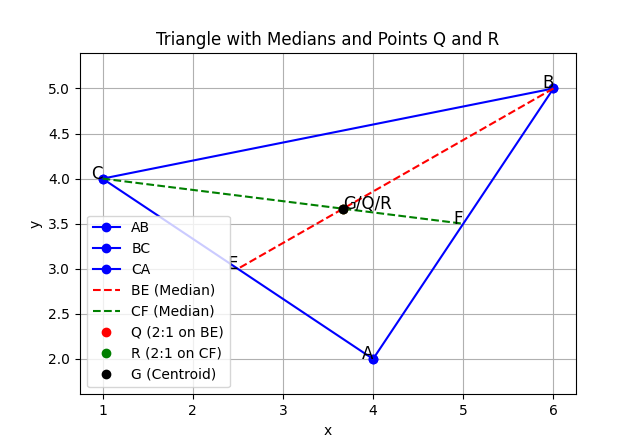
\includegraphics[width=0.7\linewidth]{Figure_1.png}
   \caption{Plot of Triangle $ABC$}
   \label{stemplot}
\end{figure}
\end{document}
